\graphicspath{{./ch_C13_dephasing_LDE/figures/}}


\chapter{Analysis of a quantum memory with optical interface in diamond }
\label{ch:CDL}

\begin{center} 
    \vspace{-1cm} {M.S.~Blok$^*$, N.~Kalb$^*$, A.~Reiserer, T.H.~Taminiau and R.~Hanson} 
\end{center}

{\renewcommand{\thefootnote}{}\footnote{This chapter has been accepted for publication in
    {\em Faraday Discussions} (2015).}\footnote{$^*$ these authors contributed equally to this work}}

\vspace{-0.5cm} 

Single defect centers in diamond have emerged as a powerful platform for quantum optics experiments and quantum information processing tasks\cite{Gao_NatPhoton_2015}. Connecting spatially separated nodes via optical photons\cite{Kimble_Nature_2008} into a quantum network will enable distributed quantum computing and long-range quantum communication. Initial experiments on trapped atoms and ions as well as defects in diamond have demonstrated entanglement between two nodes over several meters\cite{Moehring_Nature_2007,Ritter_Nature_2012,Hofmann_Science_2012,Bernien_Nature_2013}. To realize multi-node networks, additional quantum bit systems that store quantum states while new entanglement links are established are highly desirable. Such memories allow for entanglement distillation, purification and quantum repeater protocols that extend the size, speed and distance of the network\cite{Bennett_Phys.Rev.Lett._1996,Campbell_Phys.Rev.Lett._2008,Briegel_Phys.Rev.Lett._1998,Childress_Phys.Rev.Lett._2006}. However, to be effective the memory must be robust against the entanglement generation protocol, which typically must be repeated many times. Here we evaluate the prospects of using carbon nuclear spins in diamond as quantum memories that are compatible with quantum networks based on single nitrogen vacancy (NV) defects in diamond. We present a theoretical framework to describe the dephasing of the nuclear spins under repeated generation of NV spin-photon entanglement and show that quantum states can be stored during hundreds of repetitions using typical experimental coupling parameters. This result demonstrates that nuclear spins with weak hyperfine couplings are promising quantum memories for quantum networks.
\clearpage

\section{Introduction}

Spins associated with the nitrogen-vacancy (NV) center, an atomic defect in diamond, have recently emerged as a promising platform for quantum networks\cite{Gao_NatPhoton_2015,Childress__2013}. The NV-center’s long-lived electron spin state (\textit{S} = 1) can be controlled by magnetic resonance and can be initialized and read out optically. At cryogenic temperatures (< 10 K), coherent optical transitions allow for the generation of spin-photon entanglement\cite{Togan_Nature_2010} and of entanglement between spatially separated NV center electron spins\cite{Bernien_Nature_2013,Pfaff_Science_2014}. 

In addition, the electron spin couples to nuclear spins in the environment through the hyperfine interaction. Control over the host nitrogen spin and over multiple nearby $^{13}C$ spins has been demonstrated\cite{Jelezko_Phys.Rev.Lett._2004,Dutt_Science_2007,Neumann_Science_2008a,Smeltzer_Phys.Rev.A_2009,Fuchs_NatPhys_2011,vanderSar_Nature_2012,Taminiau_Phys.Rev.Lett._2012}. As these nuclear spins can be well isolated from their environments, coherence times of more than one second have been demonstrated\cite{Maurer_Science_2012}, making them interesting candidates for quantum network memories. 

A major challenge for realizing quantum memories based on nuclear spins is to overcome the dephasing that is introduced while using the electron spin as an optical interface to generate spin-photon entanglement. Consider the general case of an entanglement protocol that is inherently probabilistic due to lossy optical channels. The protocol therefore must be repeated many times in order to establish an entanglement link between adjacent network nodes. Whenever the entanglement attempt fails, the electron spin is projected in a random state. A fast and practical solution is to re-initialize the spin by optical pumping after each repetition. Because the exact time at which the electron spin is reset is uncertain (optical pumping is a stochastic process) and the electron-nuclear interaction is always present, the electron reset can cause nuclear spin dephasing (Fig \ref{fig:cdl-fig1}). A promising route to overcome this dephasing of the quantum memory is to use relatively distant $^{13}C$ spins with weak hyperfine couplings, which are less sensitive to fluctuations of the electron spin.  

In this manuscript we explore the storage of quantum states in $^{13}C$ spins during the repeated generation of NV spin-photon entanglement. We first demonstrate a method to directly measure the frequency difference \textit{df} for the electron-state-dependent nuclear spin precessions, which governs the nuclear dephasing (Fig. \ref{fig:cdl-fig1})\cite{Laraoui_NatCommun_2013}. We then analyze the spin-photon entanglement protocol, develop a model to describe the dephasing of nuclear spins, and calculate the fidelity of nuclear spin quantum memories with realistic coupling parameters under many repetitions of the entanglement protocol. 


\section{Control and Characterization of nuclear spins in diamond}
\begin{figure*}
	\centering
	\includegraphics[width=130mm]{Fig1}
	\caption{\label{fig:cdl-fig1} \textbf{The NV-center as a network node including a quantum memory} A single electron spin (orange) is coupled (purple curly arrows) to individual carbon spins (blue) via the magnetic dipole field (black dashed lines) associated with the electron spin. A laser beam (red straight arrow) is used to prepare and read-out the spin state by collecting the florescence (red curly arrow). (a) Scanning electron microscope image of the sample. A solid-immersion lens is fabricated with a focused ion beam in single-crystalline diamond for high collection efficiency. An on-chip gold stripline (bottom) enables microwave-control. (b) Level scheme for the quantum memory ($^{13}C$-spin, \textit{I} = 1/2). The hyperfine coupling introduces energy level splittings ($\omega_0$ and $\omega_1$) that depend on the state of the electron spin, where  $\omega_0$ = (2$\pi$) $\gamma_C B$ with $\gamma_C$ the gyromagnetic ratio of the carbon spin and \textit{B} the magnetic field and $\omega_1$ depends on the hyperfine coupling, which is set by the distance to the electron spin. (c) Relevant ground-state energy levels of the electron spin (\textit{S} = 1). The degeneracy of the $m_s = \pm 1$ states is lifted by applying a magnetic field along the quantization axis of the NV-center. We define the electron spin qubit in the $\ket{0} = m_s = 0$,$\ket{1} = m_s = +1$ manifold. Here $B_z$ = (303 $\pm$ 1) G leading to an energy level splitting $\omega_e \sim$ (2$\pi$) 3.73 GHz. (d) Diagram of the electron spin including the relevant ground-, and excited-state levels. At low temperature the zero phonon line ($\sim$ 637 nm)  exhibits spin-preserving optical transitions that can be addressed selectively. In the experiment, two lasers with different frequency are used to address the E’ transition for electron spin initialization (dashed red) and the $E_y$ transition for readout (fidelity = 0.93(5)) and generating spin-photon entanglement (solid red).}
\end{figure*}

We start by discussing the experimental methods to control the NV center and nearby $^{13}C$  nuclear spins. We then introduce a Ramsey-spectroscopy method to directly determine the frequency df and characterize four candidate $^{13}C$  spins near a single NV-center. These experimental results highlight the universal presence of controllable nuclear spin memories and provide a realistic set of input parameters for the theoretical calculations.

At the heart of the experiment is a single Nitrogen-Vacancy (NV) center in high purity (Type IIa) single-crystal diamond grown by chemical-vapor-deposition. The diamond is held at a temperature of \textit{T} = 4.2 K in a Helium bath cryostat. The diamond has a natural abundance (1.1\%) of $^{13}C$ spins (\textit{I} = 1/2) in an otherwise $^{12}C$ spin-free lattice. The NV electronic spin is polarized and measured optically by spin-selective resonant excitation\cite{Togan_Nature_2010,Tamarat_NewJ.Phys._2008,Robledo_Nature_2011}. To obtain high single-shot readout fidelities, a solid-immersion lens was fabricated on top of the NV center and a single-layer aluminum-oxide anti-reflective coating was deposited\cite{Pfaff_Science_2014} (Fig \ref{fig:cdl-fig1}a). The electronic spin is controlled by microwaves applied through an on-chip line (Rabi frequency: 3.3 MHz).     

We detect and control multiple $^{13}C$ nuclear spins in the spin bath surrounding the NV center using recently developed methods that coherently exploit the electron-nuclear interaction by periodically switching the electron state at well-defined times\cite{Taminiau_Phys.Rev.Lett._2012,Kolkowitz_Phys.Rev.Lett._2012,Zhao_NatNano_2012,Taminiau_NatNano_2014}. We apply sequences of the form $(\tau - \pi - 2\tau - \pi - \tau)^{M/2}$, where $\pi$ denotes a microwave pulse that rotates the electron by 180 degrees, $2\tau$ is the interpulse delay and \textit{M} the total number of $\pi$-pulses. For $\tau$ precisely resonant with the electron-nuclear dynamics, this sequence imprints a phase on the electron spin conditional on the nuclear spin state. 

\begin{figure*}
	\centering
	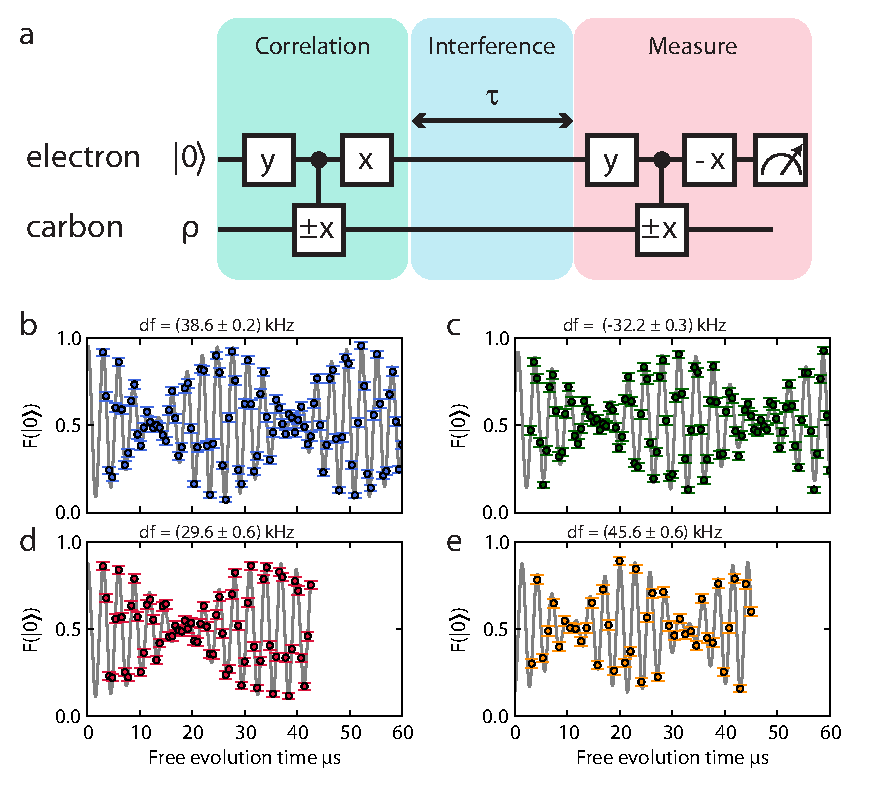
\includegraphics[width=130mm]{Fig2}
	\caption{\label{fig:cdl-fig2} \textbf{Characterization of single $^{13}C$ spins.} (a) Circuit diagram to determine $\omega_0$ and $\omega_1$ of individual $^{13}C$ spins via the electron spin. The conditional gates on the carbon spin are implemented using resonant dynamical decoupling techniques as explained in the main text. Because the evolution of the carbon spin is correlated with an eigenstate of the electron spin during the interference, a coherent signal can be observed even for $\tau \gg T^{*}_{2,electron}$ = (4.18 $\pm$ 0.01) $\mu$s (b)-(e) The resulting interference signal measured for four individual $^{13}C$ spins near a single NV-center. Grey lines are fits to the data with function $F = \frac{A}{2}\cos(\omega_0 \tau +\phi_0) + \frac{B}{2}\cos(\omega_1 \tau + \phi_1)$. We find $\omega_0$ /2$\pi$ = (326.0 $\pm$ 0.2), (325.9 $\pm$ 0.2), (325.1 $\pm$ 0.5), (325.9 $\pm$ 0.4) kHz (b-e), consistent with the gyromagnetic ratio of a $^{13}C$ spin in a field of (303 $\pm$ 1) G.  For the second frequency component we find $\omega_1$ /2$\pi$ = (364.6 $\pm$ 0.1), (293.7 $\pm$ 0.2), (354.7 $\pm$ 0.5), (371.5 $\pm$ 0.4) kHz. The data is taken with 500 repetitions per data point and the error bars correspond to one standard deviation.}
\end{figure*}

Because the hyperfine interaction is determined by the specific position of each nuclear spin relative to the NV center, the resonance condition for $\tau$ is different for each nuclear spin. We can thus characterize the nuclear spin environment\cite{Taminiau_Phys.Rev.Lett._2012} by preparing the electron in a superposition state and measuring the phase that is acquired when sweeping $\tau$. Here we select four individual $^{13}C$ spins to study in more detail, and design controlled gates following Taminiau et al.\cite{Taminiau_NatNano_2014}.

The nuclear spin dynamics are characterized by the nuclear spin precession frequencies $\omega_0$ and $\omega_1$  corresponding to the electron spin being in $m_s = 0$ and $m_s = 1$, respectively (see also Methods). To directly determine the frequencies $\omega_0$,  $\omega_1$ and $df = ( \omega_1 − \omega_0 )/2 \pi$  for each of the four nuclear spins we perform the experimental sequence\cite{Laraoui_NatCommun_2013} shown in Fig. \ref{fig:cdl-fig2}a. The electron is prepared in state $\rho_{0,e} = \ket{0}\bra{0}$, whereas the nuclear spin state is un-polarized (mixed state $\rho_{m.C} = (\ket{0}\bra{0} + \ket{1}\bra{1})/2$ ). The first set of gates correlates the electron state with the X-projection of the nuclear spin state, so that the state is $\rho_{0,e} \otimes \rho_{x,C} + \rho_{1,e} \otimes \rho_{-x,C}$ , with $\rho_{\pm X,C} = \ket{\pm X}\bra{\pm X}$ and  $\ket{\pm X} = (\ket{0}_C \pm \ket{1}_C)/\sqrt{2}$. The controlled nuclear spin rotations are realized by the pulse sequences described above, with $\tau$ resonant for that specific spin. Second, the nuclear spin evolves freely, either with $\omega_0$ or with $\omega_1$, depending on the electron state. Finally the phase accumulation of the nuclear spin is measured by correlating it to the electron spin before reading out the electron spin. 

The beating observed in the signal directly yields the frequency difference df and therefore the additional phase picked up due to the time the electron spent in $m_s = + 1$.   For the four spins we find $df = (29.6 \pm 0.6), (-32.2 \pm 0.3) (38.6 \pm 0.2)$ and $ (45.6 \pm 0.6) $  kHz respectively.  These values show that several nuclear spins with coupling strengths between approximately 20-50 kHz are readily available in diamond samples with a natural abundance of $^{13}C$.

\section{Modeling the dephasing of a carbon spin during entanglement generation}

We analyze the performance of $^{13}C$ spins as quantum memory in the context of  the  heralded entanglement protocol proposed by Barrett and Kok\cite{Barrett_Phys.Rev.A_2005}, which was implemented by Bernien et al.\cite{Bernien_Nature_2013}. The protocol is based on the creation of spin-photon entanglement at both nodes, followed by two-photon interference and measurement of these photons. The protocol is probabilistic since it is susceptible to photon loss. Importantly, successful generation of entanglement is heralded by the detection of the two photons and thus the sequence can be repeated until successful. 

Spin-photon entanglement is created using the following sequence (Fig. \ref{fig:cdl-fig3}a). The electron spin is prepared in state $\ket{0}_e$ by optical pumping (Fig. \ref{fig:cdl-fig1}d). Using microwaves the electron spin is then brought in a coherent superposition. Next, the NV center is optically excited with a short laser pulse that is only resonant if the spin is in state $\ket{0}_e$. Spontaneous emission generates a photon that is entangled with the state of the spin: $\ket{\Psi} = (\ket{0}_e \ket{1}_p +\ket{1}_e \ket{0}_p)/\sqrt{2}$  where $\ket{1}_p$ ($\ket{0}_p$)  denotes the presence (absence) of a photon. The goal is that the nuclear spin memory reliably stores quantum states during many repetitions of this sequence.

 \begin{figure*}
	\centering
	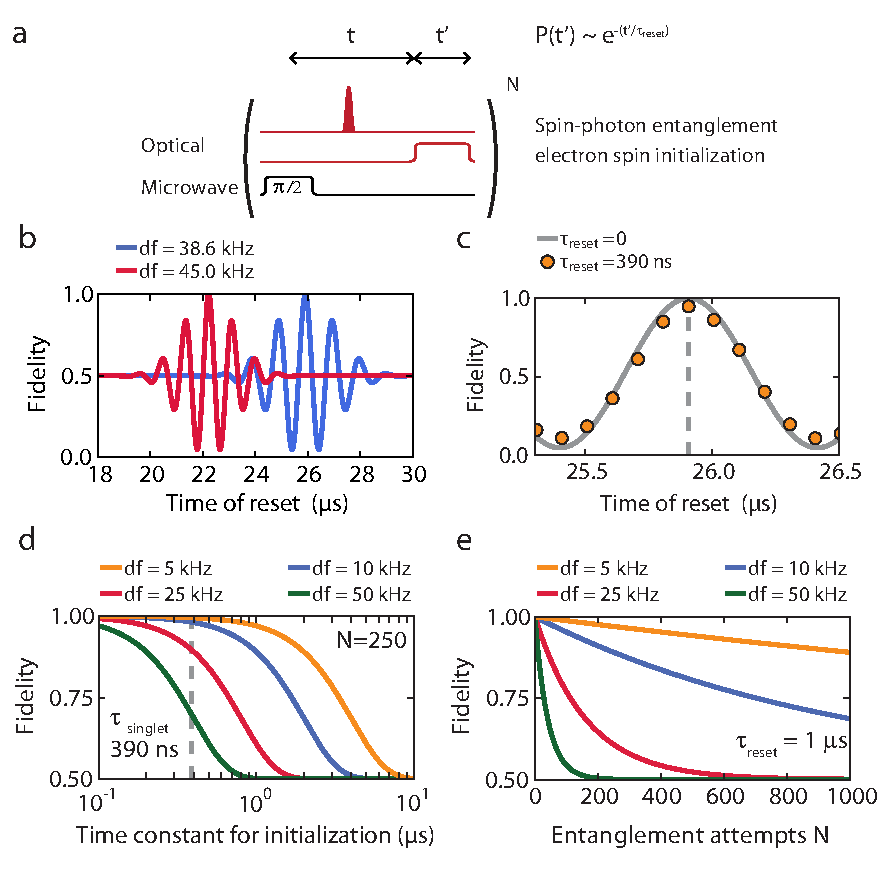
\includegraphics[width=130mm]{Fig3}
	\caption{\label{fig:cdl-fig3} \textbf{Simulations of the dephasing of a $^{13}C$ spin quantum memory while generating entanglement. } (a) Diagram for the protocol to create spin-photon entanglement. (b) Simulations of the fidelity for different $^{13}C$ spins after \textit{N} = 50 repetitions of the protocol, assuming that the reset is instantaneous ($t^{\prime}$ = 0, formula \ref{eq:CDL-deph} of main text). The initial state of a carbon spin can be perfectly preserved by choosing the time between the $\pi$/2-pulse and the reset to \textit{t} = 2$\pi$ /$d \omega$. (c) The effect of the spin pumping process on the fidelity of the memory after \textit{N} = 50 repetitions. Orange dots are a Monte-Carlo simulation where for every electron spin reset, a time $t^{\prime}$ is drawn from an exponential probability distribution with $\tau_{reset}$ = 390 ns. Grey line is a comparison with an ideal reset. $d \omega$ = (2$\pi$) 38.6 kHz. (d) Dependence of the memory fidelity on the characteristic reset time $\tau_{reset}$ using formula \ref{eq:CDL-deph_an}. (e) Dephasing of the memory as a function of entanglement attempts for different coupling strengths, fixing  $\tau_{reset}$ = 1 $\mu$s.}
\end{figure*}



The performance of a quantum memory can be characterized by its ability to store an unknown quantum state $\ket{\psi} = \alpha \ket{0}_C + \beta e^{i \phi}\ket{1}_C$. During the spin-photon entanglement sequences the phase $\phi$ of the nuclear spin state is affected in two ways. First, when the emitted photon is lost (heralding fails), the electron spin state is randomly projected into either $\ket{0}_e$ or $\ket{1}_e$ resulting in nuclear spin evolutions with $\omega_0$ or $\omega_1$, respectively. Second, before the next repetition, the electron spin is reset by optical pumping, a stochastic process that introduces a distribution of spin flip times. These two effects are now analyzed separately.

After a single round of optical excitation that generates spin-photon entanglement, the electron spin is projected into an unknown eigenstate if the photon is lost. The carbon spin acquires a phase $d \omega t$ if the electron is projected in $\ket{1}_e$, where $d \omega = 2 \pi df$ and \textit{t} the time at which the reset is applied. When this process is repeated \textit{N} times, the number of times \textit{k} that the electron is projected in $\ket{1}_e$ is given by a binomial distribution and the final state fidelity \textit{F} of the carbon spin state is given by:

\begin{equation}\label{eq:CDL-deph}
F = \frac{1}{2} + \frac{1}{2^{N+1}} \sum_{k=0}^{N} \binom{N}{k} \cos \lbrack k d \omega t \rbrack
\end{equation}

where the electron spin reset is taken to be instantaneous and we only consider the initial memory state is $\ket{\psi} = (\ket{0}_C + \ket{1}_C/\sqrt(2)$, which is most sensitive to dephasing. Fig. \ref{fig:cdl-fig3}b shows the calculated fidelity as a function of the time \textit{t}, for two carbon spins that were identified in Fig. \ref{fig:cdl-fig2}. For each carbon spin there is a unique condition at \textit{t} =2$\pi$ /$d \omega$, for which the phase is independent on the electron state resulting in \textit{F} = 1. Note that in the full entanglement protocol\cite{Bernien_Nature_2013,Barrett_Phys.Rev.A_2005} an electron $\pi$-pulse is applied between rounds of excitation, so that this phase difference can be cancelled for all \textit{t}. 


In reality the reset of the electron spin by spin pumping is a stochastic process involving multiple transitions to the optically excited state as well as mixing between multiple excited states. Here we model the dynamics of this process as an exponential distribution  $e^{- \frac{ t^{\prime} } {\tau_{reset} } }$  with a characteristic time $\tau_{reset}$.  In Fig. \ref{fig:cdl-fig3}c we compare the results of a monte-carlo simulation that includes the probabilistic reset time $t^{\prime}$ for $\tau_{reset}$ = 390 ns with the curve of equation \ref{eq:CDL-deph}. As expected the same behavior is observed, but the maximum fidelity is reduced since the stochastic reset leads to dephasing of the carbon spin. 

To analyze the effect of the electron spin reset on the nuclear spin in detail we now assume that  \textit{t} = 2$\pi$ $d\omega$ which allows us to derive an analytical expression for the fidelity of the carbon spin (see methods for the derivation of this result): 

\begin{equation}\label{eq:CDL-deph_an}
F = \frac{1}{2} + \frac{1}{2^{N+1}}\left(1 + e^{-\frac{1}{2}\tau_{reset} ^2 d\omega^2}\right)^N.
\end{equation}

In Fig. \ref{fig:cdl-fig3}d we plot the resulting memory fidelity after 250 entanglement repetitions versus the reset constant $\tau_{reset}$, for different values of \textit{df}. Although for an instantaneous reset ($\tau_{reset} \to 0$) the state can be perfectly preserved, a finite uncertainty in the reset time constant reduces the fidelity, with the effect being stronger for higher coupling strengths df. A natural lower limit to the reset time $\tau_{reset}$ is the slowest decay rate involved in the spin pumping process. For the NV center this is expected to be the singlet lifetime $\tau_{singlet} \approx$ 390 ns\cite{Doherty_PhysicsReports_2013}.  For this value, Fig. \ref{fig:cdl-fig3}d predicts that for coupling strengths of \textit{df} < 10 kHz the state can be preserved with a fidelity of > 98 \% even after 250 entanglement attempts. 

The reset constants currently reported in the literature are approximately 1 $\mu$s \cite{Bernien_Nature_2013}. In Fig. \ref{fig:cdl-fig3}e we plot the fidelity as a function of number of entanglement attempts for $\tau_{reset}$ = 1 $\mu$s. These calculations predict that 25 repetitions of the entanglement protocol will yield a fidelity of 90.3 \% for the lowest coupling strength found in Fig. \ref{fig:cdl-fig2}, which would already provide significant speed advantages in establishing entanglement links\cite{Campbell_Phys.Rev.Lett._2008}. For coupling strengths \textit{df} < 10 kHz, hundreds of repetitions become feasible. Such lower coupling strengths are available in isotopically purified diamonds\cite{Maurer_Science_2012}.

We emphasize that the model presented here does not include the detailed excited state dynamics of the spin pumping process. We expect that averaging over rapid spin flips and time spent in states with zero spin projection during these dynamics will further reduce actual dephasing. We therefore expect that our analysis sets a lower bound for the number of possible repetitions.

We have modelled the dephasing of nuclear spins quantum memories coupled to an NV electron spin that is repeatedly used to establish spin-photon entanglement. We find that nuclear spins with weak hyperfine couplings (20-50 kHz) are readily available in natural abundance diamonds. Our analysis shows that these spins can be used to store quantum states during 25 entanglement attempts with a fidelity of 90.3 \%, while nuclear spins in isotopically purified samples with coupling strengths below 10 kHz can even enable hundreds of repetitions. These results demonstrate that nuclear spins with weak hyperfine coupling strengths are promising quantum memories for quantum networks providing a route towards entanglement distillation and quantum repeaters.

\section{Methods}
We take the limit of $\gamma_C B \gg A_{\perp}$ (with $A_{\perp}$  the hyperfine component perpendicular to the static magnetic field) such that the eigenstates of the $^{13}$C-spin are independent of the electron and the only net effect of the electron-carbon coupling is that the carbon acquires a phase depending on the state of the electron. Choosing the rotating frame of the carbon resonant with the energy splitting for the electron in $\ket{0}_e$, the carbon state will acquire a phase $e^{id\omega t}$ for the electron in $\ket{1}_e$ (with $d \omega$ = 2$\pi$ \textit{df}) and does not evolve otherwise.

We derive an expression for the maximally achievable memory fidelity. The scheme of Fig 3a is repeated \textit{N} times. Phase errors occur if the electron spin has to be reinitialized by pumping it to another spin state. During every execution of the protocol, the electron spin is projected into $\ket{0}_e$ or $\ket{1}_e$ with equal probability. The probability for \textit{k} repumping events is then given by a binomial distribution

\begin{equation}
P_{ek} = \frac{1}{2^N}\binom{N}{k}
\end{equation}

Every time the electron is reset from $\ket{1}_e$ into $\ket{0}_e$ the memory spin will pick up a random phase $\delta \theta = d \omega (t^{\prime} - \tau_{reset})$ which is given by the difference between energy levels of the carbon spin conditional on the electron spin $d \omega$ and the deviation $(t^{\prime} - \tau_{reset})$ from the mean repumping time. The overall acquired phase for \textit{k}  repumping events is then the sum of the individual random phases. The fidelity with the initial memory state after \textit{N} repetitions is thus given by

\begin{equation}
F_k = \frac{1}{2}\left(1+\cos \left[\sum_{k=0}^N \delta \theta_k\right]\right)
\end{equation}

Under the assumption that the distributions for all repumping events are independent the problem can be seen as a random walk in accumulated repumping time. Each step of this random walk is then exponentially distributed around the mean repumping time $\tau_{reset}$. The probability distribution of the summed repumping time is given by\cite{Akkouchi_CCMS_2008}

\begin{equation}
P_{ek} = \frac{t'^{k-1}}{\tau_{reset}^k(k-1)! }e^{-t^{\prime}/\tau_{reset}} \approx \frac{1}{\sqrt{2\pi}\sigma}e^{-\frac{(t^{\prime}-\mu)^2}{2\sigma^2}}
\end{equation}


where we use the central limit theorem to approximate this distribution by a normal distribution with width $\sigma = \tau_{reset} \sqrt{k}$ and mean $\mu = \tau_{reset} k$ , as we are interested in solutions for a large number of repumping events. The expected fidelity after \textit{N} experimental runs is calculated by summing over the probability distributions for the electronic state and the corresponding accumulated repumping time

\begin{eqnarray}
F_N & = & \sum_{k=0}^N  P_{ek} \int F_k\, P_{ek}\, dt^{\prime} \nonumber \\
& = & \frac{1}{2} + \frac{1}{2} \sum_{k=0}^N P_{ek} e^{-\frac{1}{2}k\tau_{reset}^2 d \omega^2} \nonumber \\
& = & \frac{1}{2} + \frac{1}{2^{N+1}}\left(1 + e^{-\frac{1}{2}\tau_{reset}^2 d \omega^2}\right)^N.
\end{eqnarray}

\newpage
\bibliographystyle{../thesis}
\bibliography{cdl}


